\subsection{Manipulation Experiments on OpenML Benchmarks}
\label{sec:semi_synthetic_results}

The context-perturbation track contains 72 OpenML-CC18 classification and 35
OpenML-CTR23 regression datasets; the distribution-shift track contains 35
and 33, respectively. Clean performance uses the original context and input.

% Original sources for every named Table 1 and Table 4 predictor. The
% non-printing citations preserve the compact result layout while ensuring
% that each baseline has a corresponding bibliography entry.
\nocite{cox1958binary,hoerl1970ridge,cortes1995svm,drucker1996svr,
cover1967knn,breiman2001randomforests,ke2017lightgbm,
prokhorenkova2018catboost,chen2016xgboost,rumelhart1986backprop,
gorishniy2021fttransformer,gorishniy2025tabm,thielmann2024tabularnn,
ahamed2024mambatab,holzmueller2024realmlp,qu2026tabiclv2,
grinsztajn2026tabpfn3technicalreport,wang2026limix2m,ma2025tabdpt}

Table~\ref{tab:overall-performance} compares thirteen conventional or neural
baselines with four frozen tabular foundation models: LimiX-2M, TabICL-v2,
TabPFN-v3, and TabDPT v1.2. Relative to Base, Shared improves every nonzero
perturbation and shift metric. Specific adds a further gain in every comparison.
Clean scores remain essentially unchanged. Baseline configurations,
citations, and the full-suite LimiX compatibility protocol appear in
Appendix~\ref{app:baseline_details}.

\paragraph{Strength response on OpenML tasks.}
Figure~\ref{fig:semisynthetic-strength} reports all five strengths, equally
weighting datasets and the five perturbation or seven shift families. The
three configurations are close at strength zero. As strength increases, Base
degrades fastest, Shared consistently attenuates the decline, and Specific
improves further, achieving the best score across all eight panels at every
nonzero strength.

\subsection{Fully Synthetic Robustness}
\label{sec:results}

\paragraph{Protocol and baselines.}
We evaluate a fixed five-slot Shared interface on twelve synthetic problem
families generated by five data-generating processes with correlated features
and controlled targets. Each family is tested at five strengths and three
random seeds. Comparisons cover nine robust-learning, adversarial-training,
and distribution-adaptation baselines listed in
Appendix~\ref{app:baseline_details}. Aligned evaluation units use AUROC for
classification and $R^2$ for regression.

\ifdefined\ICLRLayout
\begin{figure}[H]
  \centering
  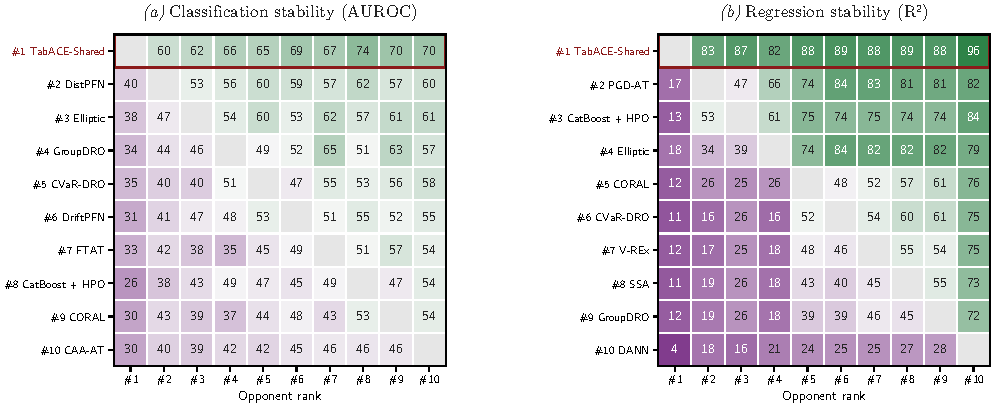
\includegraphics[width=0.88\textwidth]{figures/tabace_synthetic_stability.pdf}
  \caption{Pairwise stability over 180 aligned seed--DGP--scenario units.
  Classification uses chance-adjusted AUROC-margin degradation and regression
  uses normalized $R^2$ degradation. Cells show how often the row method has
  the smaller drop; differences within $0.001$ are ties.}
  \label{fig:synthetic-stability}
\end{figure}

\begin{figure}[H]
  \centering
  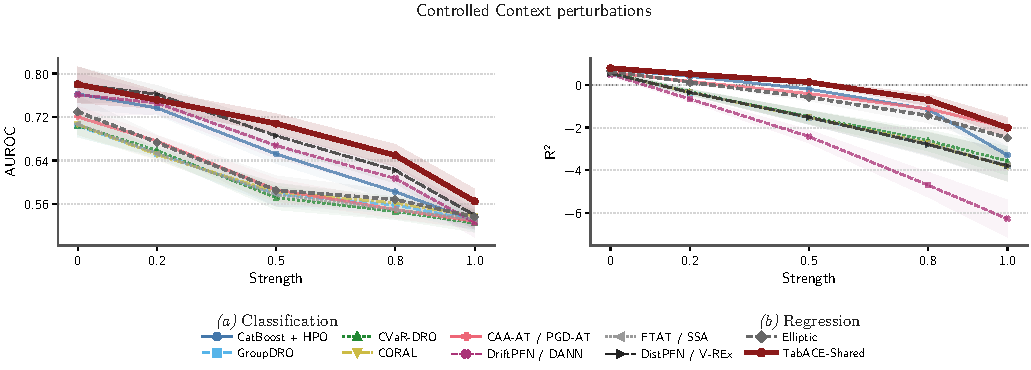
\includegraphics[width=0.94\textwidth]{figures/tabace_controlled_response.pdf}
  \caption{Fully synthetic response to controlled context perturbations.
  Panels report classification AUROC and regression $R^2$; curves pool
  aligned units over five perturbation families and bands show 95\% bootstrap
  intervals.}
  \label{fig:synthetic-controlled-response}
\end{figure}
\fi

\paragraph{Stability.}
For each seed--DGP--scenario unit, we average the four nonzero strengths and
normalize classification degradation by the clean AUROC discrimination margin
and regression degradation by the clean $R^2$. Exact definitions appear in
Appendix~\ref{app:metrics_reporting}.
Figure~\ref{fig:synthetic-stability} reports pairwise win rates over 180
aligned units. TabACE-Shared ranks first in both classification and regression,
with mean win rates of 67.0\% and 87.6\%, respectively.

\ifdefined\ICLRLayout
\paragraph{Strength response.}
Figure~\ref{fig:synthetic-controlled-response} reports classification AUROC
and regression $R^2$ under controlled context perturbations. Curves equally
weight aligned DGP, problem, and seed units and show 95\% bootstrap intervals.
TabACE-Shared attains the highest classification AUROC from strength $0.5$
onward. The context-count and aggregation ablations appear in the appendix.

\subsection{Additional Experiments}
\label{sec:additional-experiments}

\paragraph{Natural distribution shifts.}
Folktables~\citep{ding2021folktables} provides a 2018
California-to-Michigan geographic shift and a 2014-to-2018 temporal shift
within California. Table~\ref{tab:natural-shifts} reports ID and OOD Accuracy
for Employment, Income, and TravelTime. Specific achieves the highest score in
every setting.

\providecolor{revisionblue}{RGB}{25,55,135}
\definecolor{sharedblue}{RGB}{31,84,147}
\definecolor{specificred}{RGB}{213,94,0}

\begin{table}[H]
  \centering
  \begin{minipage}[t]{0.61\textwidth}
    \vspace{0pt}
    \centering
    \caption{ID and OOD Accuracy under natural geographic and temporal shifts.}
    \label{tab:natural-shifts}
    \small
    \setlength{\tabcolsep}{4.0pt}
    \renewcommand{\arraystretch}{1.02}
    \begin{tabular}{@{}llccc@{}}
      \toprule
      Method & Domain & Employment & Income & TravelTime \\
      \midrule
      \multicolumn{5}{@{}l}{\textit{Geographic: California $\rightarrow$ Michigan (2018)}} \\
      Base & ID  & 0.7922 & 0.7888 & 0.5912 \\
           & OOD & 0.8043 & 0.7655 & 0.5472 \\
      Shared & ID
        & \textcolor{revisionblue}{0.7952} & \textcolor{revisionblue}{0.8118}
        & \textcolor{revisionblue}{0.6225} \\
           & OOD
        & \textcolor{revisionblue}{0.8106} & \textcolor{revisionblue}{0.7823}
        & \textcolor{revisionblue}{0.5818} \\
      Specific & ID
        & \textcolor{revisionblue}{\textbf{0.8089}}
        & \textcolor{revisionblue}{\textbf{0.8201}}
        & \textcolor{revisionblue}{\textbf{0.6569}} \\
           & OOD
        & \textcolor{revisionblue}{\textbf{0.8245}}
        & \textcolor{revisionblue}{\textbf{0.7914}}
        & \textcolor{revisionblue}{\textbf{0.6012}} \\
      \addlinespace[2pt]
      \multicolumn{5}{@{}l}{\textit{Temporal: California 2014 $\rightarrow$ 2018}} \\
      Base & ID  & 0.7704 & 0.7926 & 0.5951 \\
           & OOD & 0.7847 & 0.7844 & 0.5908 \\
      Shared & ID
        & \textcolor{revisionblue}{0.7861} & \textcolor{revisionblue}{0.8126}
        & \textcolor{revisionblue}{0.6237} \\
           & OOD
        & \textcolor{revisionblue}{0.7922} & \textcolor{revisionblue}{0.8000}
        & \textcolor{revisionblue}{0.6045} \\
      Specific & ID
        & \textcolor{revisionblue}{\textbf{0.7994}}
        & \textcolor{revisionblue}{\textbf{0.8240}}
        & \textcolor{revisionblue}{\textbf{0.6526}} \\
           & OOD
        & \textcolor{revisionblue}{\textbf{0.8030}}
        & \textcolor{revisionblue}{\textbf{0.8106}}
        & \textcolor{revisionblue}{\textbf{0.6350}} \\
      \bottomrule
    \end{tabular}
  \end{minipage}\hfill
  \begin{minipage}[t]{0.36\textwidth}
    \vspace{0pt}
    \centering
    \caption{Gains over each unmodified conventional predictor from context ensembling.}
    \label{tab:traditional-backbone-gains}
    \small
    \setlength{\tabcolsep}{4.0pt}
    \renewcommand{\arraystretch}{1.02}
    \begin{tabular}{@{}lcc@{}}
      \toprule
      \multicolumn{3}{c}{Classification: $\Delta$Accuracy $\uparrow$} \\
      \cmidrule(lr){1-3}
      Predictor & Shared & Specific \\
      \midrule
      kNN & \textcolor{sharedblue}{+0.0167}
        & \textcolor{specificred}{\textbf{+0.0227}} \\
      Logistic & \textcolor{sharedblue}{+0.0069}
        & \textcolor{specificred}{\textbf{+0.0287}} \\
      CatBoost & \textcolor{sharedblue}{+0.0145}
        & \textcolor{specificred}{\textbf{+0.0287}} \\
      MLP & \textcolor{sharedblue}{+0.0107}
        & \textcolor{specificred}{\textbf{+0.0285}} \\
      \addlinespace[5pt]
      \multicolumn{3}{c}{Regression: $\Delta R^2$ $\uparrow$} \\
      \cmidrule(lr){1-3}
      Predictor & Shared & Specific \\
      \midrule
      kNN & \textcolor{sharedblue}{+0.0203}
        & \textcolor{specificred}{\textbf{+0.0654}} \\
      Ridge & \textcolor{sharedblue}{+0.1425}
        & \textcolor{specificred}{\textbf{+0.1966}} \\
      CatBoost & \textcolor{sharedblue}{+0.1279}
        & \textcolor{specificred}{\textbf{+0.1740}} \\
      MLP & \textcolor{sharedblue}{+0.0499}
        & \textcolor{specificred}{\textbf{+0.1645}} \\
      \bottomrule
    \end{tabular}
  \end{minipage}
\end{table}


\begin{figure}[H]
  \centering
  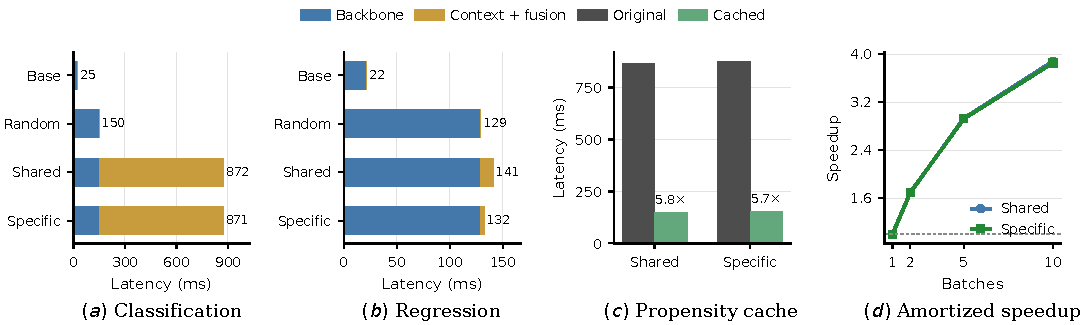
\includegraphics[width=0.96\textwidth]{figures/tabace_inference_cost_ablation.pdf}
  \caption{Inference-cost ablation under a fixed budget of five alternative
  contexts for both Shared and Specific, with a separately evaluated Base
  branch. Panels (a--b) decompose median latency; (c) compares original and
  cached inference; (d) includes the one-time cache setup in the amortized
  speedup.}
  \label{fig:inference-cost}
\end{figure}
\else
\paragraph{Strength response.}
Figure~\ref{fig:synthetic-controlled-response} reports classification AUROC
and regression $R^2$ under controlled context perturbations. Curves equally
weight aligned DGP, problem, and seed units and show 95\% bootstrap intervals.
TabACE-Shared attains the highest classification AUROC from strength $0.5$
onward. The context-count and aggregation ablations appear in the appendix.
\fi

\ifdefined\ICLRLayout\else
\subsection{Additional Experiments}
\label{sec:additional-experiments}

\paragraph{Natural distribution shifts.}
Folktables~\citep{ding2021folktables} provides a 2018
California-to-Michigan geographic shift and a 2014-to-2018 temporal shift
within California. Table~\ref{tab:natural-shifts} reports ID and OOD Accuracy
for Employment, Income, and TravelTime. Specific achieves the highest score in
every setting.
\fi

\paragraph{Conventional-predictor compatibility.}
Applying the same context-ensemble interface to kNN, Logistic/Ridge, CatBoost,
and MLP improves classification Accuracy and regression $R^2$ for every
predictor with Shared, while Specific adds a further gain in all eight
comparisons (Table~\ref{tab:traditional-backbone-gains}).

\paragraph{Inference cost.}
Figure~\ref{fig:inference-cost} fixes both Shared and Specific to five
alternative contexts for a matched-cost comparison; this coincides with the
fixed Shared bank. The figure decomposes wall-clock latency into six backbone
passes (Base plus five alternatives) and context construction/fusion. Caching
reusable propensity quantities yields about $5.7\times$ faster repeated
inference. After including the one-time cache construction, it retains about
$3.9\times$ amortized speedup over ten batches.

\FloatBarrier
